\documentclass{beamer}
\usetheme{Madrid}
\usepackage{graphicx}
\usepackage{amsmath}
\usepackage{booktabs}
\usepackage{hyperref}

\title[MELANIN ON MARGINS]{Melanin on Margins: A Study on Skin-Color Bias in the Bollywood Film Industry}
\author{Abhik Rana\\ (\textbf{BS2301})}
\date{May 2025}

\begin{document}
% Title Slide
\begin{frame}
    \titlepage
\end{frame}

% Slide 1: Introduction
\begin{frame}{Introduction}
    \begin{itemize}
        \item Bollywood reaches over 90 countries with a \$2.1B market.
        \item Despite this reach, there is limited research on colorism in casting.
        \item This study investigates how skin tone bias manifests in Hindi cinema.
    \end{itemize}
\end{frame}

% % Slide 2: Research Questions
\begin{frame}{Research Questions}
  \begin{enumerate}
    \item How pronounced is colorism in Bollywood movies?
    \item How has colorism changed over time?
    \item What is the distribution of skin tones across roles?
    \item What are the average luminance trends?
  \end{enumerate}
\end{frame}

% % Slide 3: Data Collection
\begin{frame}{Data Set}
  \begin{itemize}
    \item Top 5 grossing movies each year (2015--2024).
    \item Extracted L* values from CIELAB color space.
    \item Leading and supporting cast analyzed separately by gender.
    \item Average luminance used as proxy for skin tone.
  \end{itemize}
\end{frame}

% % Slide 4: Preprocessing
\begin{frame}{Dataset Cleaning and Preprocessing}
  \begin{itemize}
    \item Selected scenes with visible glabella.
    \item Removed outliers and standardized frame counts.
    \item Averaged support cast L* values per scene.
    \item Manual filtering of foreign or heavily made-up faces.
  \end{itemize}
\end{frame}

% % Slide 5: ANOVA - Concept
\begin{frame}{ANOVA: Concept}
  \begin{itemize}
    \item Used to compare L* across four roles:
    \begin{itemize}
      \item actor, actress, side\_actor, side\_actress
    \end{itemize}
    \item Hypothesis:
    \[ H_0: \mu_\text{actor} = \mu_\text{actress} = \mu_\text{side\_actor} = \mu_\text{side\_actress} \]
    \item Tested via F-statistic:
    \[ F = \frac{\text{between-group variance}}{\text{within-group variance}} \]
  \end{itemize}
\end{frame}

% % Slide 6: ANOVA Results
\begin{frame}{ANOVA Results}
  \begin{table}[]
    \centering
    \begin{tabular}{lrrrr}
    \toprule
    Source & sum\_sq & df & F & PR(>F) \\
    \midrule
    C(role) & 26213.77 & 3 & 117.25 & $1.63 \times 10^{-43}$ \\
    Residual & 14606.09 & 196 & & \\
    \bottomrule
    \end{tabular}
    \caption{ANOVA for Luminance by Role}
  \end{table}
  \small Null hypothesis rejected: at least one role differs significantly in average luminance.
\end{frame}

% % Slide 7: ANOVA by Year
\begin{frame}{ANOVA: Luminance by Year}
  \begin{table}[]
    \centering
    \begin{tabular}{lrrrr}
    \toprule
    Source & sum\_sq & df & F & PR(>F) \\
    \midrule
    C(year) & 1458.47 & 9 & 0.78 & 0.63 \\
    Residual & 39361.40 & 190 & & \\
    \bottomrule
    \end{tabular}
    \caption{ANOVA for Luminance by Year}
  \end{table}
  \small No significant difference across years.
\end{frame}

% % Slide 8: Cohen's d
\begin{frame}{Cohen's d Effect Size}
  \begin{itemize}
    \item Formula: \( d = \frac{L_A - L_B}{s_{\text{pooled}}} \)
    \item Actor vs Actress: \( d = -2.319 \) (actors significantly lighter)
    \item Lead vs Side roles: \( d = 1.492 \) (leads significantly lighter)
  \end{itemize}
\end{frame}

% % Slide 9: Distribution Overview
\begin{frame}{Distribution of Skin Tones}
  \begin{itemize}
    \item Multiple visualizations to assess role-based luminance differences.
    \item Next slides show KDEs, histograms, percentiles, and trends.
  \end{itemize}
\end{frame}

% % Slide 10: Luminance Distribution by Role
\begin{frame}{Luminance Distribution by Role}
  \centering
  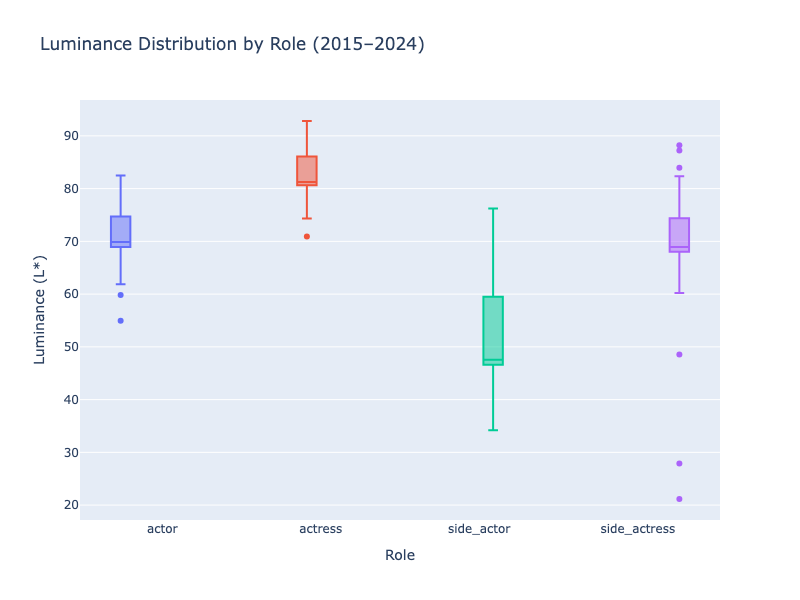
\includegraphics[width=0.85\textwidth]{figures/luminance_distribution_by_role.png}
\end{frame}

% % Slide 11: Histogram
\begin{frame}{Luminance Histogram by Role}
  \centering
  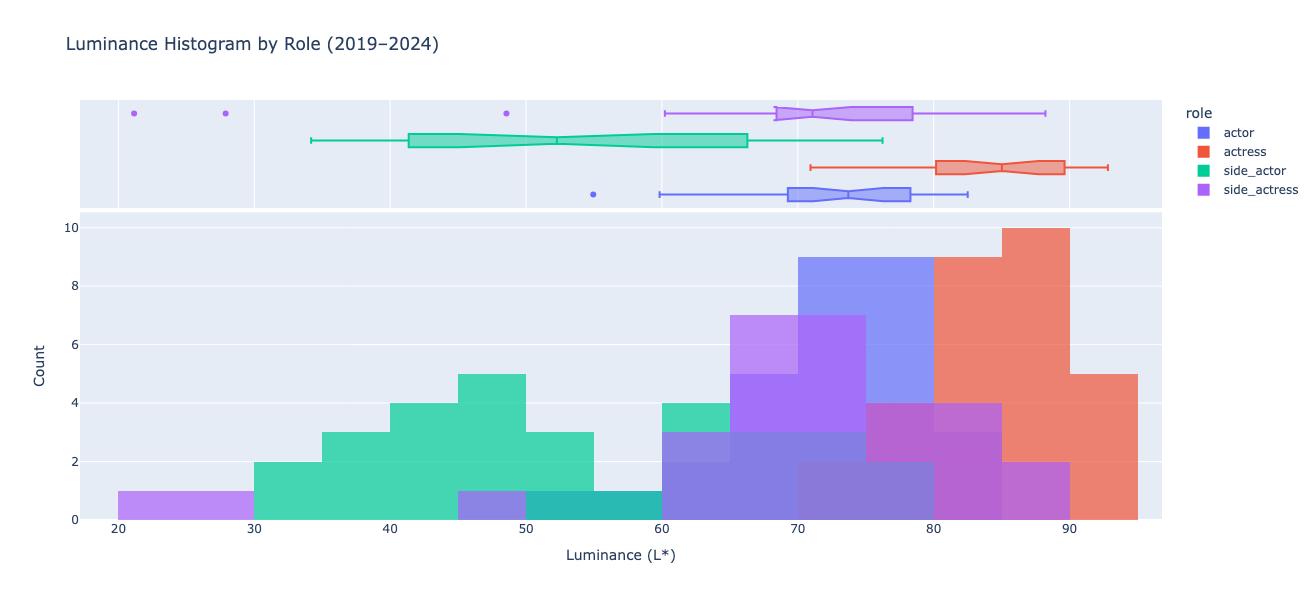
\includegraphics[width=0.85\textwidth]{figures/luminance_histogram_by_role.png}
\end{frame}

% % Slide 12: Percentile Overlay
\begin{frame}{Luminance Distribution with Percentiles}
  \centering
  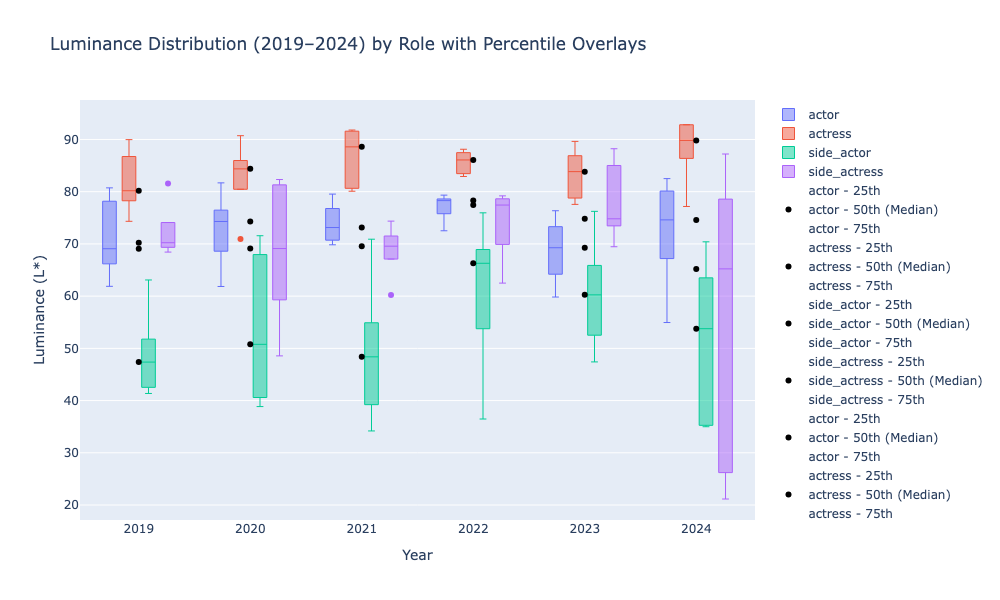
\includegraphics[width=0.85\textwidth]{figures/luminance_distribution_by_role_with_percentile_overlays.png}
\end{frame}

% % Slide 13: Avg Over Time
\begin{frame}{Average Luminance Over Time by Role}
  \centering
  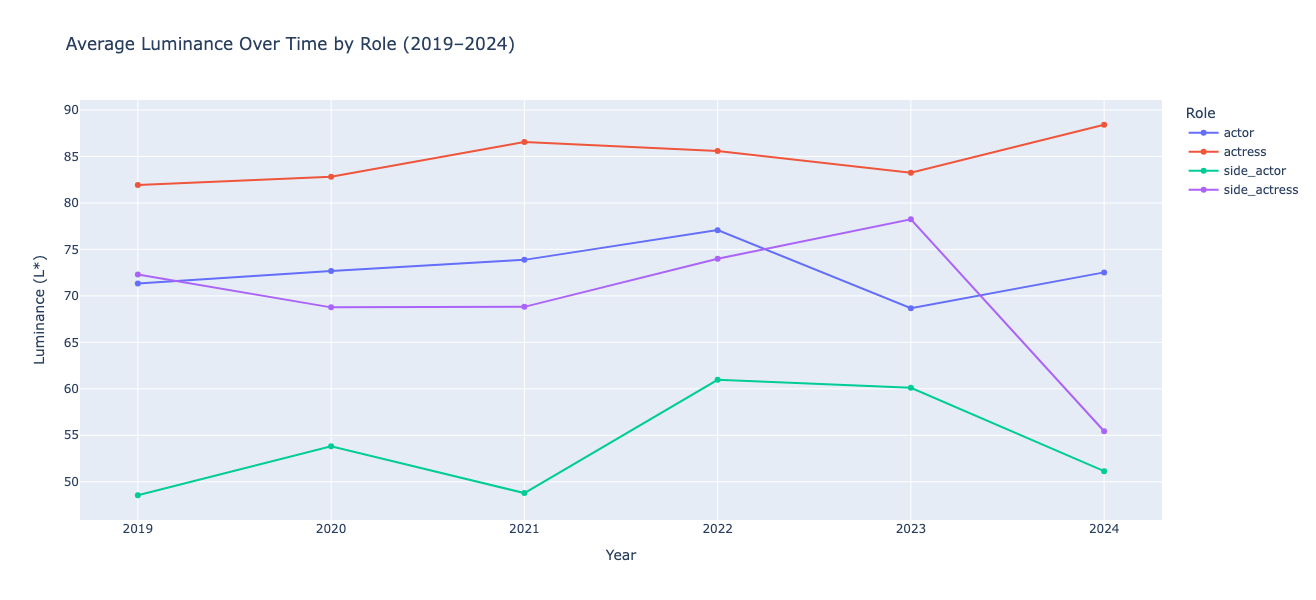
\includegraphics[width=0.85\textwidth]{figures/average_luminance_over_time_by_role.png}
\end{frame}

% % Slide 14: Observed Trends
\begin{frame}{Observed Trends}
  \begin{itemize}
    \item Persistent preference for lighter skin in lead roles.
    \item Clustering and trendline analyses support earlier findings.
  \end{itemize}
\end{frame}

% % Slide 15: Linear Trend Plot
\begin{frame}{Linear Trend of Luminance by Role}
  \centering
  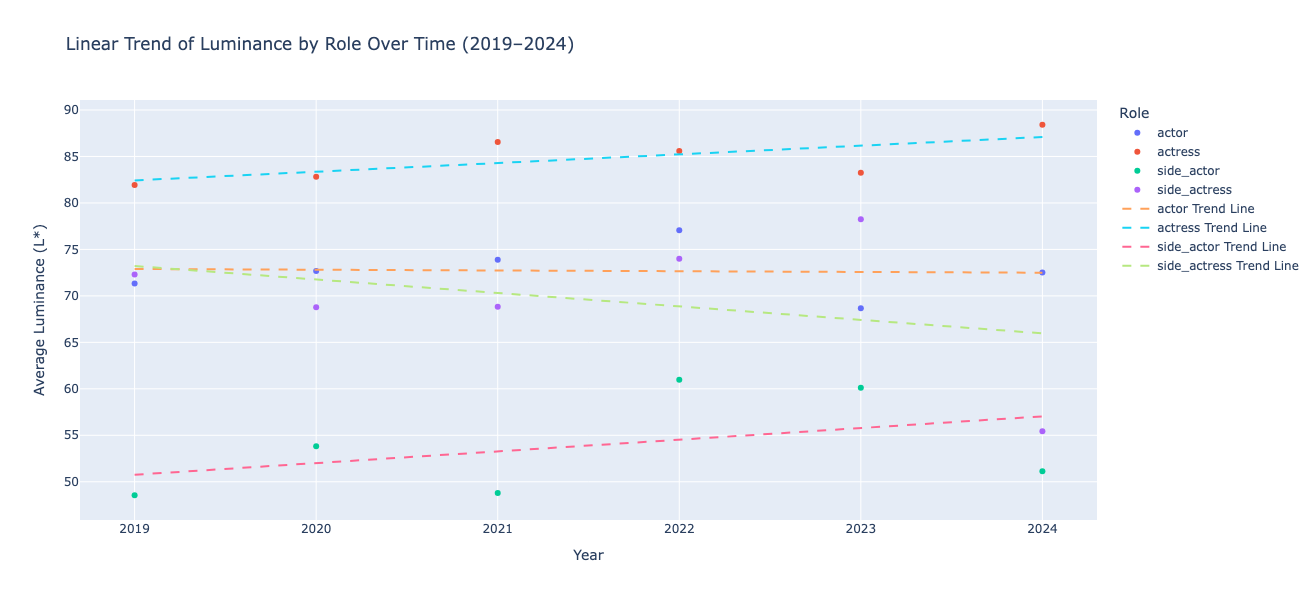
\includegraphics[width=0.85\textwidth]{figures/linear_trand_of_luminance_by_role.png}
\end{frame}

% % Slide 16: K-Means Clustering
\begin{frame}{K-Means Clustering of Luminance}
  \centering
  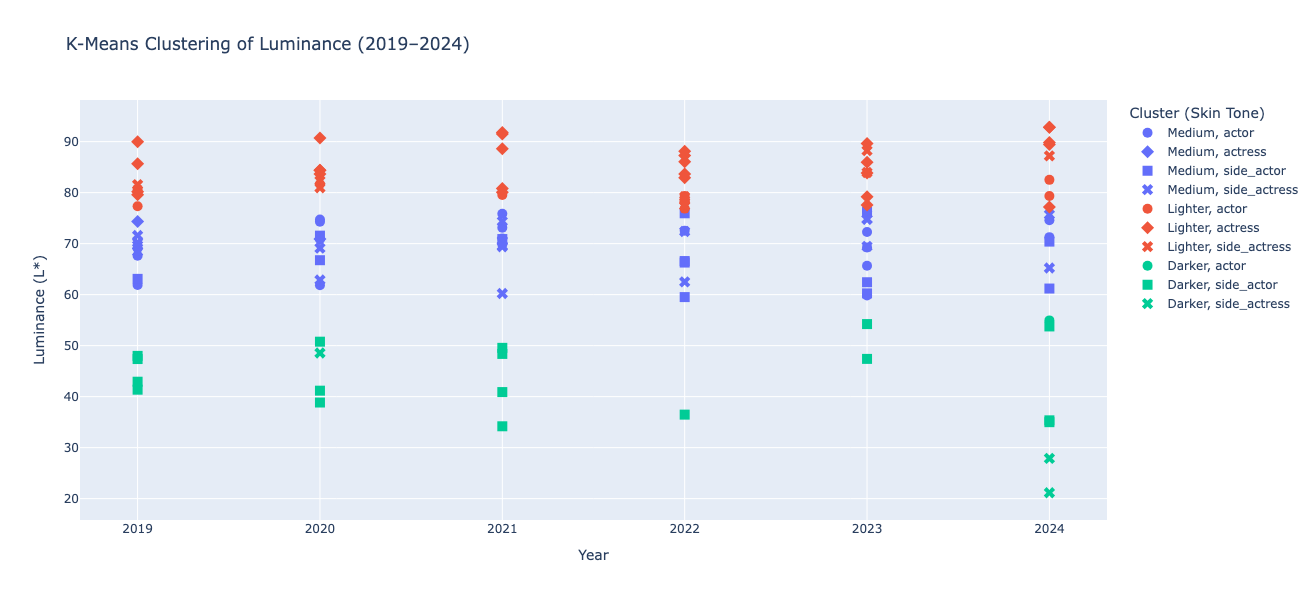
\includegraphics[width=0.85\textwidth]{figures/k_means_clustering.png}
\end{frame}

% % Slide 17: Interpretation
\begin{frame}{Clustering Interpretation}
  \begin{itemize}
    \item Cluster 0: Darker tones $\rightarrow$ More side roles.
    \item Cluster 2: Lighter tones $\rightarrow$ Mostly lead roles.
    \item Supports presence of colorism through unsupervised learning.
  \end{itemize}
\end{frame}

% % Slide 18: Conclusion
\begin{frame}{Conclusion}
  \begin{itemize}
    \item Strong empirical evidence of colorism.
    \item Leads have significantly lighter skin than supporting characters.
    \item Temporal trends show little progress.
    \item Statistical and ML methods converge on similar findings.
  \end{itemize}
\end{frame}

% % Slide 19: Acknowledgments
\begin{frame}{Acknowledgments}
  I would like to express my sincere gratitude to \\ 
  \textbf{Professor Garga Chatterjee} and \textbf{Professor Kuntal Ghosh} \\ 
  for their invaluable guidance and mentorship throughout this study.
\end{frame}

% % Slide 20: Thank You
\begin{frame}{Thank You}
  \centering
  \Huge Questions?
\end{frame}

\end{document}
